% !TeX root = ../main.tex

\chapter{相关理论和技术介绍}

在本章中,我们回顾一下实现编译器所需的基本工具。
程序通常由程序员以文本形式输入,即字符序列。程序作为文本的表示称为具体语法。
我们用具体语法简明地写下和讨论程序的语法。
在编译器中,我们使用抽象语法树来表示程序,因为编译器可以很方便高效地操作抽象语法树。
翻译具体语法到抽象语法的过程称作解析。
本文不涉及解析的理论和实现,一方面是因为现阶段解析已经有了相对固定化的套路和工具,研究也已经趋于完善。
另一方面由于本文选择了 Racket 作为源语言和实现语言,我们可以很方便地从字符串序列中构造出结构体,
而 Racket 的结构体也是本文选择的用以表示抽象语法树的数据结构。

\section{抽象语法树}

在计算机科学中,抽象语法树,或简称语法树,是源代码语法结构的一种抽象表示。
它以树状的形式表现编程语言的语法结构,树上的每个节点都表示源代码中的一种结构。
之所以说语法是“抽象”的,是因为这里的语法并不会表示出真实语法中出现的每个细节。
比如,嵌套括号被隐含在树的结构中,并没有以节点的形式呈现;
而类似于 if-condition-then 这样的条件跳转语句,可以使用带有三个分支的节点来表示。

\section{文法}

编程语言可以被看作是合法程序的集合,这一集合通常是无限大的,因为我们总是可以写出更加庞大复杂的程序。
因此,我们无法简单地通过把所有的合法程序列出来来描述一门语言。
通常,我们使用文法——一系列规则,来构造程序。文法通常用来描述具体语法,但它也可以被用来描述抽象语法。
本文使用巴科斯-诺尔范式\cite{Knuth_1964, Backus_Bauer_1960}的变体来描述我们的语言。
图\ref{fig:con-syntax-eg}中的几条规则给出了本文实现的语言的一个子集的描述,
该语言仅支持包含加减法的整数运算,但它允许任意复杂的嵌套表达式。

\begin{figure}[t]
  \fbox{
    \begin{minipage}{0.96\textwidth}
      \[
      \begin{array}{rcl}
        \Type & ::= & \key{Integer} \\
        \Exp & ::= & \Int \MID \LP\key{read}\RP \MID \LP\key{-}\;\Exp\RP \MID \LP\key{+} \; \Exp\;\Exp\RP \\
        \Lang & ::= & \Exp
      \end{array}
      \]
    \end{minipage}
  }
  \caption{具体语法示例}
  \label{fig:con-syntax-eg}
\end{figure}

\begin{figure}[t]
  \fbox{
    \begin{minipage}{0.96\textwidth}
      \[
      \begin{array}{rcl}
        \Type & ::= & \key{Integer} \\
        \Exp &::=& \INT{\Int} \MID \READ{} \MID \NEG{\Exp} \\
        &\MID&  \ADD{\Exp}{\Exp}  \\
        \LangInt{}  &::=& \PROGRAM{\code{'()}}{\Exp}
      \end{array}
      \]
    \end{minipage}
  }
  \caption{抽象语法示例}
  \label{fig:abs-syntax-eg}
\end{figure}

其中 \code{read} 函数读取用户在键盘上输入的一串数字,返回一个整数。
下面这行代码是这个示例语言一个完整的合法的程序:

\begin{lstlisting}
(+ (read) (- 8))
\end{lstlisting}

该程序对应的语法树如图\ref{fig:ast-eg}。

\begin{figure}[t]
  \begin{center}
      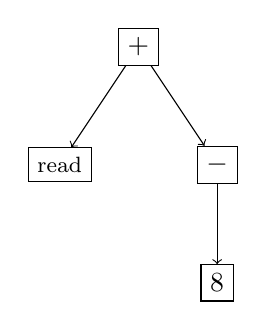
\begin{tikzpicture}
        \node[draw] (plus)  at (0 ,  0) {\key{+}};
        \node[draw] (read)  at (-1, -1.5) {{\footnotesize\key{read}}};

        \node[draw] (minus) at (1 , -1.5) {$\key{-}$};
        \node[draw] (8)     at (1 , -3) {\key{8}};

        \draw[->] (plus) to (read);
        \draw[->] (plus) to (minus);
        \draw[->] (minus) to (8);
      \end{tikzpicture}
  \end{center}
  \caption{语法树示例}
  \label{fig:ast-eg}
\end{figure}

\section{Racket 结构体和模式匹配}

图\ref{fig:con-syntax-eg}对应的抽象语法的描述如图\ref{fig:abs-syntax-eg}所示。
其中\code{Int},\code{Prim}等即为对应的Racket结构体的构造函数。
这些结构体可以非常简单地被定义出来:
\begin{lstlisting}
(struct Int (value))
(struct Prim (op args))
\end{lstlisting}

构造结构体也非常简单,下面这行代码对应的即为具体语法为\code{(+ (read) (- 8))}的程序:
\begin{lstlisting}
(Prim '+
      (list (Prim 'read '())
            (Prim '- (list (Int 8))))
\end{lstlisting}

而对结构体使用模式匹配,我们可以很方便地判断结构体的类型以及访问结构体的成员,以及语法树的子树。
例如,对于下面这段代码
\begin{lstlisting}
(match ast
  [(Prim op (list child1 child2))
   (print op)])
\end{lstlisting}
将对变量\code{ast}进行模式匹配,如果变量是一个包含两个(可能复杂的)操作数的语法树,就打印操作符。
同时,这段代码还会将两个操作数,也就是两个子树,分别绑定到变量\code{child1}和\code{child2}上去。
例如,如果\code{ast}的值是\code{(+ (read) (- 8))},
则\code{child1}和\code{child2}的值将分别被赋值为\code{(read)}和\code{(- 8)},
并且代码将打印出\code{+}。

一个模式匹配当然也可能包含多个子句,这些子句将会从上到下依次被判断是否匹配。
例如,下面这个\code{leaf?}函数接受一个名为ast的参数,判断该它是否是叶子节点:
如果是一个数字或者\code{read}函数,则为叶子节点;如果是加运算或者取负运算,则不是叶子节点。
\begin{lstlisting}
(define (leaf? ast)
  (match ast
    [(Int n) true]
    [(Prim 'read '()) true]
    [(Prim '- (list e1)) false]
    [(Prim '+ (list e1 e2)) false]))
\end{lstlisting}

以下三行代码的返回值将分别为 \code{true, false, true}:
\begin{lstlisting}
(leaf (Prim 'read '()))
(leaf (Prim '- (list (Int 8))))
(leaf (Int 8))
\end{lstlisting}

\section{源语言功能介绍}

在语言特性的选择上,我们主要考虑让它们能尽可能地体现不同的编译原理的知识面。
对于基本数据类型,本文实现了 64 位整数及其加、减、乘、整除、模运算,布尔类型及其与、或运算;
本文没有实现浮点数与浮点运算,因为它们只是单纯地覆盖了更多的 x86-64 指令,
并不会增加语言的表现力;
本文没有采用纯函数式的方式,而是支持了可变变量和循环,
因为这会迫使我们在进行数据流分析时考虑循环数据流;
对于复合数据结构,本文仅实现了元组,这足以让我们考虑堆上的内存数据和垃圾回收;
最后是函数,本文实现了一等函数,利用元组实现了闭包,并且在翻译过程中正确地处理了尾递归。

在类型系统方面,本文没有实现类型推导,但只有函数的形式参数以及返回值需要显式声明类型,
其余变量(即局部变量)定义时并不需要声明类型。例如,如下的代码是一个合法的程序。
\begin{lstlisting}
(define (even? [x : Integer]) : Boolean
  (let ([r (remainder x 2)])
    (if (eq? r 0)
        true
        false)))
\end{lstlisting}

\section{x86-64 汇编语言}

本文使用 GNU 汇编器要求的 AT\&T x86-64 汇编语法。程序以 main 标签开始,后面跟着一系列指令。
globl 指令表明 main 过程是外部可见的,这是操作系统可以调用它的必要条件。
x86 程序存储在计算机的内存中。就本文的目的而言,计算机的内存是 64 位地址到 64 位值的映射。
计算机在 rip 寄存器中存储一个程序计数器 (PC) ,它指向下一条要执行的指令的地址。
对于大多数指令,程序计数器在指令执行后递增,因此它指向内存中的下一条指令。
大多数 x86 指令有两个操作数,每个操作数要么是一个整型常量 (称为立即数) ,
要么是一个寄存器 ,要么是一个内存位置。

寄存器是一种特殊的变量,每一个都有一个 64 位的值;
计算机中有 16 个通用寄存器,它们的名称在图
%\ref{fig:full-x86}
中给出。
我们使用 \% 符号后跟寄存器名,比如 \%rax,来指代某一个寄存器。

立即数使用语法 \$n 来指明,其中 n 是整数。
访问内存使用语法 n(\%r) 来指明,它的意思是拿到存储在寄存器 r 中的地址,然后给地址加 n 个字节。

\subsection{x86 程序示例}

我们来看一个简单但完整的 x86-64 程序示例。该程序计算式子\code{(+ 52 (- 10))}的值,
并将结果作为整个程序的返回值。

\begin{lstlisting}
start:
movq	$10, -8(%rbp)
negq	-8(%rbp)
movq	-8(%rbp), %rax
addq	$52, %rax
jmp conclusion

.globl main
main:
pushq	%rbp
movq	%rsp, %rbp
subq	$16, %rsp
jmp start
conclusion:
addq	$16, %rsp
popq	%rbp
retq
\end{lstlisting}

这个程序使用一个称为过程调用栈 (简称栈) 的内存区域。
堆栈由每个过程调用的独立帧组成。单个帧的内存布局如图\ref{fig:frame}所示。
寄存器 rsp 被称为堆栈指针 ,它指向堆栈顶部的项。
堆栈在内存中向下增长,通过减去堆栈指针来增加堆栈的大小。
在过程调用的上下文中,返回地址是调用方调用指令之后的指令。
函数调用指令 callq 在跳转到过程之前将返回地址压入堆栈。
寄存器 rbp 是 基指针 ,用于访问存储在当前过程调用帧中的变量。
调用者的基指针在返回地址之后被压入堆栈,然后基指针被设置为旧基指针的位置。
变量 1 存储在地址 −8(\%rbp) ,变量 2 存储在地址 −16(\%rbp) ,以此类推。

\begin{figure}[t]
	\centering
	\begin{tabular}{|r|l|} \hline
		位置 & 内容 \\ \hline
		8(\key{\%rbp}) & return address \\
		0(\key{\%rbp}) & old \key{rbp} \\
		-8(\key{\%rbp}) & variable $1$ \\
		-16(\key{\%rbp}) & variable $2$ \\
		\ldots  & \ldots \\
		0(\key{\%rsp}) & variable $n$\\ \hline
	\end{tabular}

	\caption{栈帧的内存布局}
	\label{fig:frame}
\end{figure}

回到这个程序,首先,操作系统发出一个 callq main 指令,
将其返回地址推送到堆栈上,然后跳转到 main 。
在 x86-64 中,堆栈指针 rsp 在执行任何 callq 指令之前必须整除 16 个字节。
因此当控制到达 main 时,rsp 偏离对齐 8 个字节 (因为 callq 压入返回地址)。

前三条指令是一个程序典型的准备工作。
指令 \code{pushq \%rbp} 将调用者的基指针保存到堆栈上,并从堆栈指针中减去 8 。
第二个指令 \code{movq \%rsp, \%rbp} 读取 rsp 中的内容,赋值给 rbp。
这条指令改变了基指针,使其指向旧基指针的位置。
指令 \code{subq \$16, \%rsp} 读取 rsp 中的内容,减去 16,再重新赋值给 rsp。
这条指令将堆栈指针向下移动,以便为存储变量留出足够的空间。

虽然这个程序只需要在栈上存储一个变量 (8 个字节) ,但是我们还是需要减去 16,
这样 rsp 是 16 字节对齐的,就可以调用其他函数。
准备工作的最后一条指令是 \code{jmp start},
它使程序跳转到由 Racket 表达式 \code{(+ 52 (- 10))} 生成的指令,也就是 start 标签下的指令。

start 标签下的第一条指令是 \code{movq \$10, -8(\%rbp)},
它将 10 存储在图\ref{fig:frame}中 variable 1 的位置。
指令 \code{negq -8(\%rbp)} 将值更改为 −10。下一条指令将 \%rax 中值更改为 -10。
最后,\code{addq \$52, \%rax} 将 52 加到 rax 上,将其值更新为 42。
我们总是约定将程序的返回值放在寄存器 rax 中。

conclusion 标签下的三个指令是一个程序典型的结束工作。
前两条指令将 rsp 和 rbp 寄存器恢复到过程开始时的状态。
指令 \code{addq \$16, \%rsp} 将栈指针移回指向旧的基指针。
然后 \code{popq \%rbp} 把旧基指针返回给 rbp,并在堆栈指针上加 8。
最后一条指令 retq 返回到调用它的过程,并在堆栈指针上加 8。

\subsection{x86 中的函数调用}

x86 提供标签,以便可以引用指令的位置,这是跳转指令所需要的。
标签也可以用来标记函数指令的开头。
我们还可以通过使用 leaq 指令和 PC 相对寻址来获得一个标签的地址。
例如,下面这条指令把 add 函数的地址放入 rbx 寄存器中。
\begin{lstlisting}
  leaq add1(%rip), %rbx
\end{lstlisting}

指令指针寄存器 rip,也就是程序计数器始终指向要执行的下一条指令。
当与一个标签结合时,如\code{add1(\%rip)},
链接器计算 add1 标签的地址与 rip 此刻的位置之间的距离 d,
然后将 \code{add1(\%rip)} 更改为 \code{d(\%rip)},
通过这种方式在运行时计算出 add1 标签的地址。

由于支持一等函数,也就是将函数当作普通的变量,函数可能会被赋值给其他变量。
也就是说,某个变量中存放的可能是一个函数地址,调用这个变量就相当于调用函数,
亦即间接函数调用。对应的 x86 指令是接受一个寄存器名的 callq* 指令:
\begin{lstlisting}
  callq *%rbx
\end{lstlisting}

callq 指令为实现函数提供了部分支持:它将返回地址压入堆栈,
然后跳转到目标函数。但是 callq 不处理:
\begin{enumerate}
\item 参数传递
\item 把帧压入过程调用栈以及取出或访问它们
\item 确定不同函数如何共享寄存器
\end{enumerate}

函数调用需要两段代码之间的协调,这两段代码可能由不同的程序员编写或由不同的编译器生成。
这里我们遵循 Linux 和 MacOS 上的 GNU C 编译器使用的
System V 调用约定\cite{Matz_Hubicka_Jaeger_Mitchell_2013}。
调用约定包括关于函数如何共享寄存器使用的规则。
特别是,调用方负责在函数调用之前释放一些寄存器,供被调用方使用。
这些被称为“调用者保存寄存器”,它们是
\begin{lstlisting}
rax rcx rdx rsi rdi r8 r9 r10 r11
\end{lstlisting}
另一方面,被调用方负责保留“被调用者保存寄存器”,即
\begin{lstlisting}
rsp rbp rbx r12 r13 r14 r15
\end{lstlisting}

我们可以从调用方视角和被调用方视角两个角度来考虑这个调用约定:
\begin{itemize}
\item 调用方应该假定所有调用者寄存器都可以被被调用方用任意值重写。
另一方面,调用者可以安全地假设所有调用者保存的寄存器在调用后包含与调用前相同的值。
\item 被调用方可以自由地使用调用者保存寄存器。
如果被调用方希望使用被调用者保存寄存器,
被调用方必须在返回到调用方之前将原始值放回寄存器中。
这可以通过在准备工作中将值保存到调用栈中,并在函数的结束工作中恢复来实现。
\end{itemize}

在 x86 中,寄存器还用于向函数传递参数和保存返回值。
函数的前六个参数按以下顺序,在以下六个寄存器中传递。

\begin{lstlisting}
rdi rsi rdx rcx r8 r9
\end{lstlisting}

多余的参数则保存在调用方的栈帧上。
寄存器 rax 则用于函数的返回值。
